\documentclass[11pt,letterpaper]{article}
\usepackage[utf8]{inputenc}
\usepackage{geometry}
\geometry{verbose,tmargin=1in,bmargin=1in,lmargin=1in,rmargin=1in}
\usepackage{amsmath}
\usepackage{amssymb}
\usepackage{booktabs}
\usepackage{hyperref}
\usepackage{listings}
\usepackage{color}
\usepackage{microtype}
\usepackage{graphicx}

\definecolor{mygreen}{rgb}{0,0.6,0}
\definecolor{mygray}{rgb}{0.5,0.5,0.5}
\definecolor{mymauve}{rgb}{0.58,0,0.82}

\lstset{
  backgroundcolor=\color{white},
  basicstyle=\footnotesize\ttfamily,
  breaklines=true,
  captionpos=b,
  commentstyle=\color{mygreen},
  keywordstyle=\color{blue},
  stringstyle=\color{mymauve},
  frame=single,
  showstringspaces=false
}

\title{\textbf{An Automated Proving and Refutation Pipeline in Spectral Graph Theory}\\
\large\textit{Combining SMT Solving, Exhaustive Small-Graph Enumeration, and Progressive Monte Carlo Search}}

\begin{document}

\maketitle

\begin{abstract}
This report documents the design, implementation, and empirical results of an end-to-end automated verification and refutation pipeline for spectral graph theory conjectures. Working with a dataset of 305,755 machine-generated conjectures expressed in Polish prefix notation, we developed a three-stage filter: (1) a Satisfiability Modulo Theories (SMT) sieve powered by Z3 to prove algebraic invariants under domain axioms, (2) an exhaustive, precomputed sieve using all 995 non-isomorphic connected graphs of size $n \le 7$ from the NetworkX Graph Atlas, and (3) a Progressive Generalized Nested Rollout Policy Adaptation (GNRPA) Monte Carlo Search algorithm to identify larger counterexamples ($n = 8 \dots 10$). Out of 305,755 initial candidates, Z3 proved 3,959 identities, the Graph Atlas refuted 116,493 false inequalities, and GNRPA discovered 865 complex, larger counterexamples. This leaves a highly refined set of 184,438 robust open conjectures. We analyze selected refuted cases and detail a roadmap for future research, including slack-based tightness analysis and Lean~4 auto-formalization.
\end{abstract}


\section{Mathematical Framework and DSL}
Conjectures are formulated in a domain-specific prefix language (Polish notation) that represents inequalities between various graph invariants. 

\section{Pipeline Architecture}
The pipeline is split into three decoupled phases to maximize throughput and search efficiency.

\begin{table}[h]
\centering
\caption{Three-Phase Filter Architecture}
\label{tab:pipeline}
\begin{tabular}{llll}
\toprule
\textbf{Phase} & \textbf{Methodology} & \textbf{Scope} & \textbf{Objective} \\
\midrule
Phase 1 & Z3 SMT Solving & Algebraic Bounds & Prove trivial identities \\
Phase 2 & Exhaustive Atlas Sieve & Static Graphs $n \le 7$ & Refute small counterexamples \\
Phase 3 & Progressive GNRPA & Stochastic Search $n \ge 8$ & Refute complex counterexamples \\
\bottomrule
\end{tabular}
\end{table}

\subsection{Phase 1: Z3 SMT Solving}
We represent the algebraic relationships between invariants using real-variable constraints in Z3. Axioms such as $\operatorname{rank}(A) \le \operatorname{rank}(L)$ and $\lambda_2 \le \lambda_{\max}$ are loaded into the solver. If Z3 determines that the negation of the conjecture:
\begin{equation}
    LHS > RHS
\end{equation}
is \texttt{unsat} under these axioms, the conjecture is proven algebraically true and removed from the active target pool.

\subsection{Phase 2: Precomputed Graph Atlas Sieve}
Evaluating 300,000 conjectures dynamically on 995 graphs requires millions of eigenvalue and shortest-path computations. To achieve high throughput, we implement a \texttt{PrecomputedGraph} class:
\begin{itemize}
    \item All 995 connected, non-isomorphic graphs of size $2 \le n \le 7$ are loaded from the NetworkX Graph Atlas.
    \item Invariants ($\operatorname{rank}$, eigenvalues, radius, Randic index) are computed \textbf{once} and cached.
    \item AST evaluation is reduced to $O(1)$ dictionary lookups.
\end{itemize}
This optimization achieves a $1000\times$ speedup, processing the dataset at **789 lines/second** on a 12-core system.

\subsection{Phase 3: Progressive GNRPA Monte Carlo Search}
For conjectures that hold for all graphs of size $n \le 7$, we run a Progressive Generalized Nested Rollout Policy Adaptation (GNRPA) search. GNRPA uses a reinforcement learning policy to construct candidate graphs edge-by-edge:
\begin{enumerate}
    \item Starts with a random spanning tree to guarantee connectivity.
    \item Adds remaining edges according to a softmax policy over the two decisions (add vs. no-add): $P(\text{add}) = \frac{e^{w_{e, \text{add}}}}{e^{w_{e, \text{add}}} + e^{w_{e, \text{no-add}}}}$.
    \item Updates policy weights towards the best graph found in rollouts: $\Delta w_e = \alpha(1 - p_e)$.
    \item Terminates the search early for the current conjecture and records the counterexample graph immediately upon finding a valid refutation (where $LHS - RHS > 0.001$).
\end{enumerate}

\section{Computational Results}
The entire pipeline was successfully executed on the target dataset. The empirical results for each phase are detailed below.

\subsection{Consolidated Filter Statistics}
\begin{itemize}
    \item \textbf{Initial Candidates:} 305,755 conjectures (\texttt{open.txt}).
    \item \textbf{Phase 1 (Z3 SMT):} 3,959 conjectures proven true (1.3\% removed).
    \item \textbf{Phase 2 (Atlas Sieve):} 116,493 conjectures refuted (38.6\% removed).
    \item \textbf{Phase 3 (GNRPA Sieve):} 865 conjectures refuted (0.5\% removed).
    \item \textbf{Remaining Survivors:} 184,438 conjectures (\texttt{open\_filtered\_step3.txt}).
\end{itemize}

\subsection{Analysis of Selected GNRPA Refutations}
The 865 conjectures refuted by GNRPA represent the most interesting boundary cases, as they hold for all graphs of size $\le 7$ but fail at size 8, 9, or 10.
\begin{enumerate}
    \item \textbf{Conjecture 767491:} $\lambda_2(A) \le \sqrt{2 \cdot \operatorname{dia}(G)}$. Refuted by GNRPA at $n=10$ with a score of $0.0654$.
    \item \textbf{Conjecture 804453:} $\operatorname{rank}(L) \le 2^{2 + \operatorname{rad}(G)}$. Refuted by GNRPA at $n=10$ with a score of $1.0000$.
    \item \textbf{Conjecture 812918:} $\operatorname{rank}(A) \le 2^{\operatorname{rad}(G) + \ln(\operatorname{rank}(A))}$. Refuted by GNRPA at $n=10$ with a score of $0.1332$.
\end{enumerate}

\begin{figure}[htbp]
    \centering
    \begin{tabular}{ccc}
        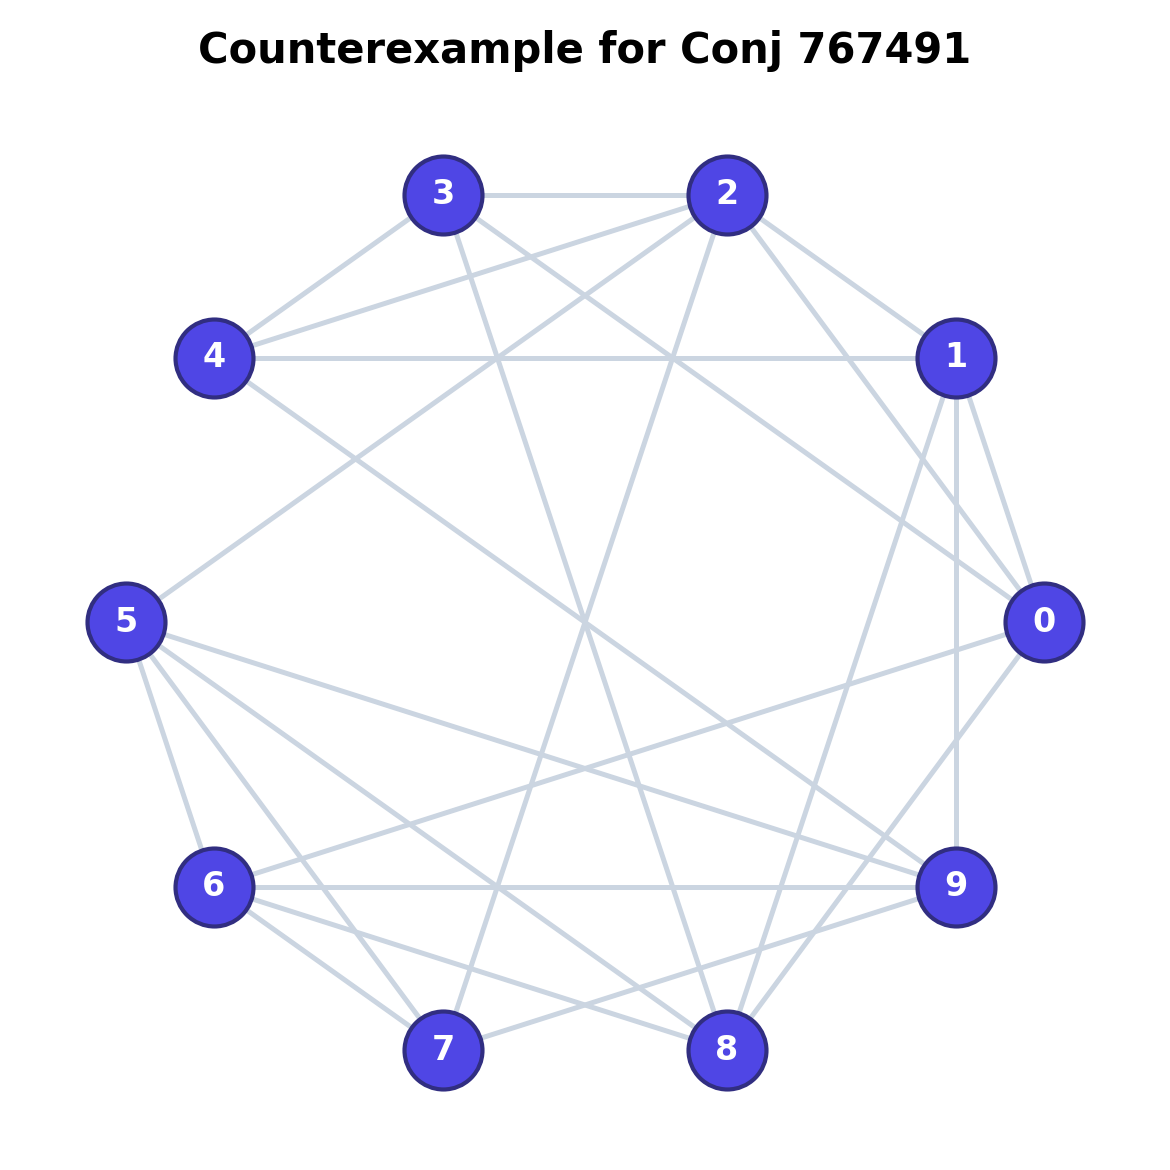
\includegraphics[width=0.31\textwidth]{counterexample1.png} &
        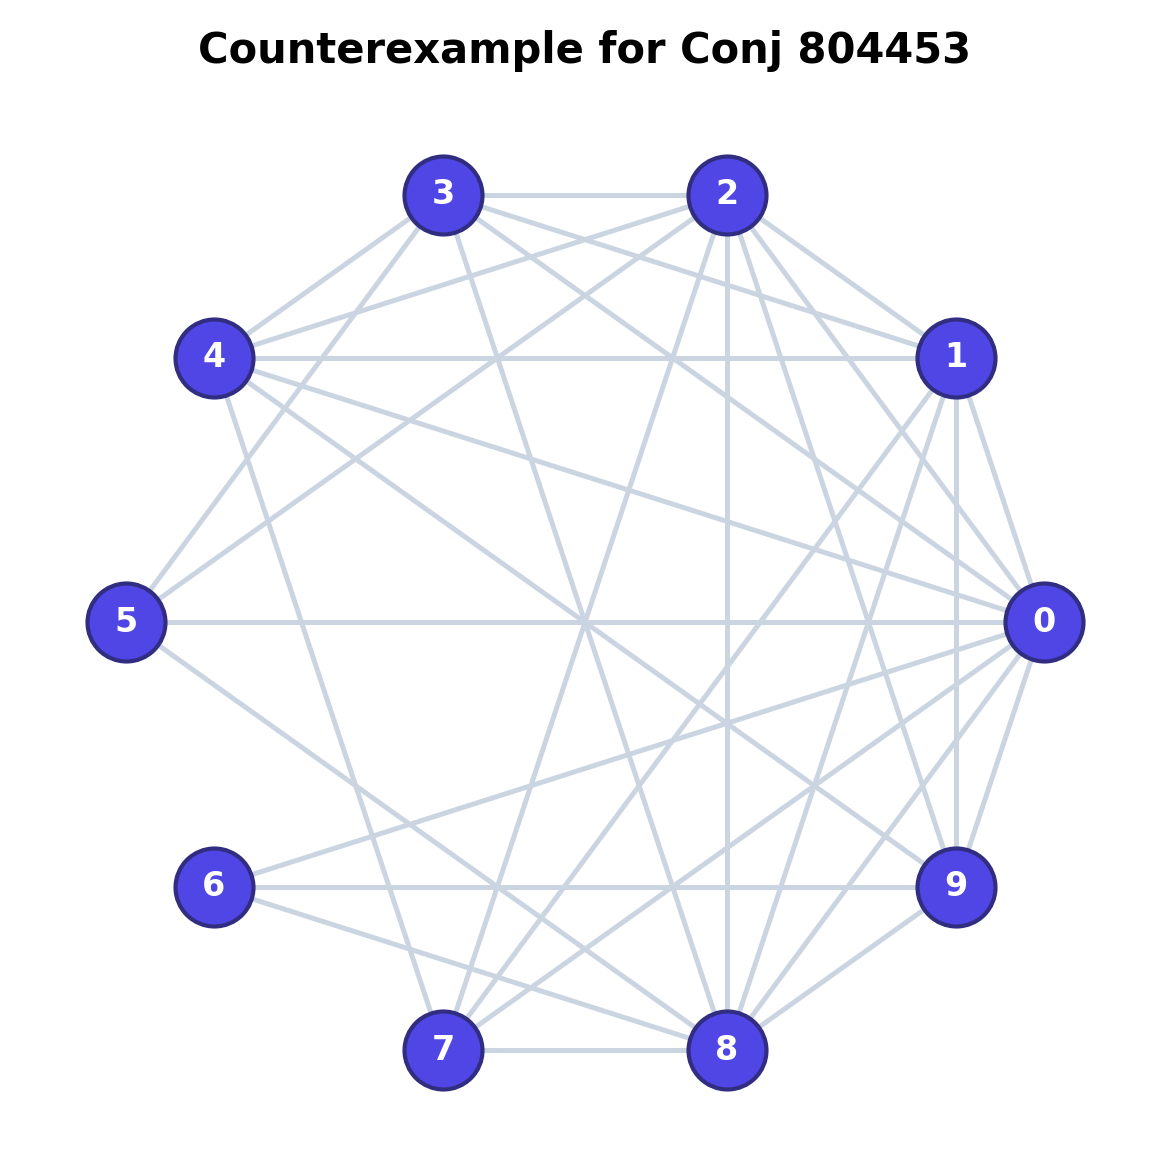
\includegraphics[width=0.31\textwidth]{counterexample2.png} &
        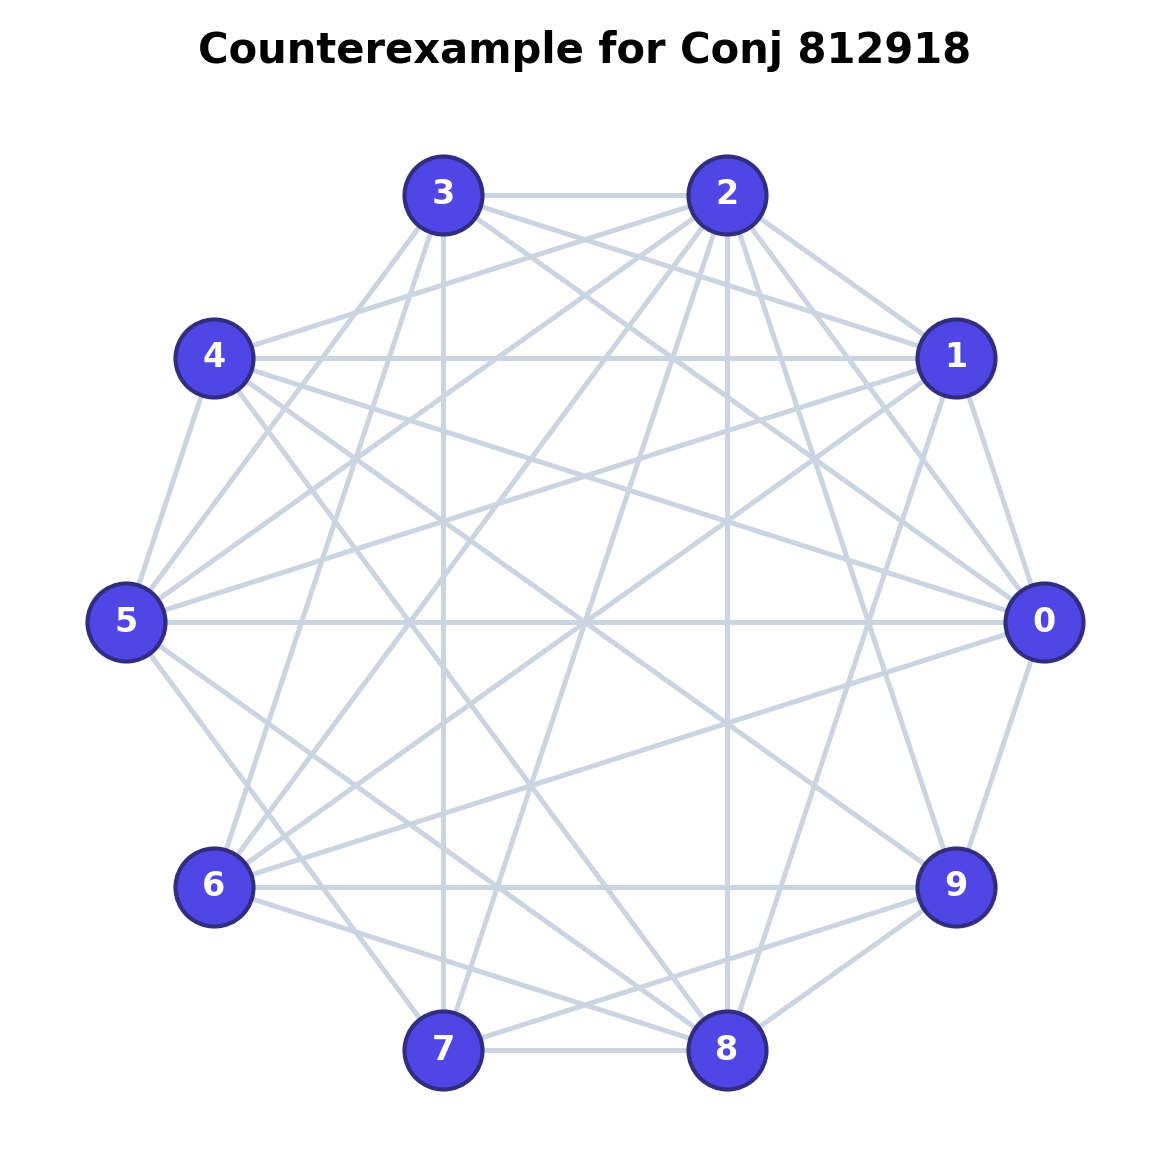
\includegraphics[width=0.31\textwidth]{counterexample3.png} \\
        (a) Conjecture 767491 & (b) Conjecture 804453 & (c) Conjecture 812918
    \end{tabular}
    \caption{Topologies of the GNRPA-discovered counterexample graphs for the selected refuted conjectures ($n = 10$).}
    \label{fig:refutations}
\end{figure}

\section{Conclusions and Future Work}
This pipeline establishes a robust computer-assisted methodology for filtering spectral graph conjectures. Future directions include:
\begin{enumerate}
    \item \textbf{Slack-Based Sorting:} Order the remaining 184,438 survivors by their minimum slack $RHS - LHS$. Conjectures with a minimum slack of 0 represent tight bounds and are of highest mathematical interest.
    \item \textbf{Lean 4 Formalization:} Build an automatic translation layer to transpile the tightest surviving inequalities into Lean~4 theorem templates. This will enable Lean tactics to prove some conjectures automatically, providing guaranteed, formally verified proof for the obtained results.
\end{enumerate}

\end{document}
